\documentclass{beamer}

\usepackage[polish]{babel}
\usepackage[utf8]{inputenc}
\usepackage[T1]{fontenc}
\usepackage{hyperref}
\usepackage{graphicx}
\usepackage{multicol}
\usepackage{tabularx}

\mode<presentation>{\usetheme{Dresden}}
\setbeamercovered{dynamic}

\title{some title}
\author{Robert Boczek \and Dawid Ciepliński}
\date{26.10.2010}

\AtBeginSection[]
	{
		\begin{frame}<beamer>
		\frametitle{Outline}
		\tableofcontents[currentsection]
		\end{frame}
	}


\begin{document}

\begin{frame}

	\titlepage

\end{frame}


\section{Architecture}

	\subsection{Overview}

		\begin{frame}{Layers and responsibility}

			\begin{figure}[H]
				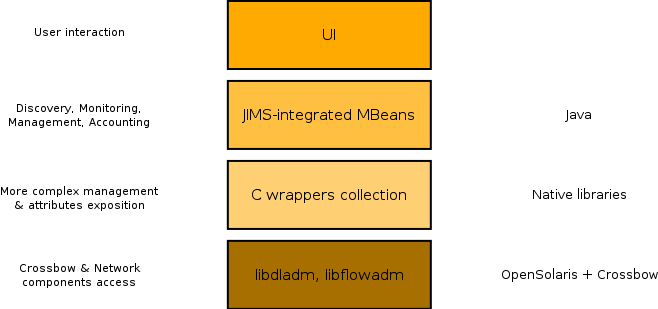
\includegraphics[width=\textwidth]{img/layers.png}
			\end{figure}
			
		\end{frame}
	

	\subsection{Layers}

		\begin{frame}{lib*adm}

			Crossbow Project libraries.

			\begin{itemize}
				\item \texttt{libdladm} provides API to manipulate VNICs, etherstubs and NICs
				\item \texttt{libflowadm} allows flow management (descriptors - e.g. addresses, protocols, ports, QoS - flow priority and maximum bandwidth)
			\end{itemize}

			Simple operations: \texttt{dladm\_set\_flowprop}, \texttt{dladm\_vnic\_delete}, etc.

		\end{frame}
	

		\begin{frame}{Native wrappers}

			Exploit Crossbow lower-level *adm libraries to provide more complex functionality.
			
			\medskip

			3 modules: \texttt{xbow-native-lib-etherstub}, \texttt{xbow-native-lib-flow}, \texttt{xbow-native-lib-link}.

			\begin{itemize}
				\item \texttt{create\_etherstub}
				\item \texttt{get\_properties}
				\item \texttt{plumb}
			\end{itemize}

		\end{frame}
	

		\begin{frame}{MBeans}

			Two kinds of objects:
			
			\begin{itemize}

				\item managers (EterstubManager, FlowManager, (V)NicManager)

					entity discovery, creation, deletion

				\item entities (flows, etherstubs, V(NIC)s)

					\begin{itemize}
						\item per-instance attributes management and monitoring
						\item hierarchy reflected in naming (e.g. MBean for \texttt{flow0}
						      created over \texttt{e1000g0} link is registered as \texttt{<domain>:type=Flow,link=e1000g0,name=flow0})
					\end{itemize}
			
			\end{itemize}

			Most often 1:1 MBean method : Native function mapping with return code to exception translation.

		\end{frame}


		\begin{frame}{User Interface}
		\end{frame}


\section{Technical issues}

	\begin{frame}{Development and code quality}

		\begin{itemize}
			\item Java and native builds with maven
			\item Unit tests \& mocks for both MBean and native code
			\item Code coverage reports
		\end{itemize}
	
	\end{frame}


\section{Roadmap}

	\begin{frame}{Roadmap}
		
		\begin{itemize}

			\item DONE
			
				C wrappers, MBeans layer $\rightarrow$ management and monitoring possible with JConsole

			\item ONGOING
			
				JIMS integration, collecting statistics

			\item FUTURE
			
				User Interface, QoS-aware zone migration

		\end{itemize}

	\end{frame}



\end{document}


% vim: enc=utf8 :
